% This is samplepaper.tex, a sample chapter demonstrating the
% LLNCS macro package for Springer Computer Science proceedings;
% Version 2.21 of 2022/01/12
%
\documentclass[runningheads]{llncs}
%
\usepackage[T1]{fontenc}
% T1 fonts will be used to generate the final print and online PDFs,
% so please use T1 fonts in your manuscript whenever possible.
% Other font encondings may result in incorrect characters.
%
\usepackage{graphicx}
\usepackage{amsmath}
\usepackage{booktabs}   % for nice tables
\usepackage{algorithm}
\usepackage{algpseudocode}
\usepackage{tabularx}
\usepackage{booktabs}
\usepackage{listings} % check to use recommended package
\usepackage[colorlinks=true, linkcolor=blue, urlcolor=cyan,
pdfpagemode=UseOutlines]{hyperref} % check if it is correct to use
% this
\hypersetup{bookmarksdepth=4}
% Manage acronyms
\usepackage[nolist]{acronym}
\usepackage{dirtytalk}
\usepackage{mismath}
\usepackage{amsmath}
\usepackage{amssymb}
% \usepackage{tikz}
% \usetikzlibrary{shapes.geometric, arrows.meta, positioning}
\usepackage{numprint}
\usepackage{multirow}

% Used for displaying a sample figure. If possible, figure files should
% be included in EPS format.
%
% If you use the hyperref package, please uncomment the following two lines
% to display URLs in blue roman font according to Springer's eBook style:
%\usepackage{color}
%\renewcommand\UrlFont{\color{blue}\rmfamily}
%\urlstyle{rm}
%

% ==================== IMRAD ====================
% 1. **I**ntroduction  
% 2. **M**ethods  
% 3. **R**esults  
% 4. **A**nd  
% 5. **D**iscussion  

% ==================== General Writing Tips ====================

% - Keep sentences clear and direct.
% - Use past tense for methods/results, present tense for facts.
% - Avoid redundancy; be precise with terminology.
% - Quantify performance improvements clearly.

% ==================== Prompts ====================
% You are computer science PhD professional. Your task is to assist me
% to improve the writing of scientific articles using academic tone and
% solving questions I have. The article is written in Latex so mastery
% in the use of Latex is expected.

\begin{document}
% Setting acronyms in paper
\begin{acronym}
  \acro{BC}[BC]{Breast Cancer}
  \acro{MG}[MG]{Mammography}
  \acro{TG}[TG]{Thermography}
  \acro{CAD}[CAD]{computer-aided detection}
  \acro{CNNs}[CNNs]{convolutional neural networks}
  \acro{ViTs}[ViTs]{Vision Transformers}
  \acro{ViT}[ViT]{Vision Transformer}
  \acro{FDA}[FDA]{Food and Drug Administration}
  \acro{SIT}[SIT]{Static Infrared Thermography}
  \acro{DIT}[DIT]{Dynamic Infrared Thermography}
  \acro{SLR}[SLR]{Systematic Literature Review}
  \acro{PICOC}[PICOC]{Population, Intervention, Comparison, Outcome,
    Context}
  \acro{DL}[DL]{Deep Learning}
  \acro{AI}[AI]{Artificial Intelligence}
  \acro{NLP}[NLP]{Natural Language Processing}
  \acro{TCN}[TCN]{Temporal Convolutional Network}
  \acro{TDL}[TDL]{Time Distributed Layers}
  \acro{RNN}[RNN]{Recurrent Neural Networks}
  \acro{HAR}[HAR]{Human Activity Recognition}
  \acro{ViViTs}[ViViTs]{Video Vision Transformers}
  \acro{ViViT}[ViViT]{Video Vision Transformer}
  \acro{IR}[IR]{Infrared Images}
  \acro{TM}[TM]{Temperature Maps}
  \acro{LSTM}[LSTM]{Long Short Memory}
\end{acronym}

% 
% \title{Transformer-based Breast Cancer Thermography Detection} 
\title{Video Transformers for Dynamic Breast Infrared Imaging Classification}
%
%\titlerunning{Abbreviated paper title}
% If the paper title is too long for the running head, you can set
% an abbreviated paper title here
%
\author{Lenin G. Falconi\inst{1}\orcidID{0000-0003-4402-6643} \and
Maria G. Perez\inst{1}\orcidID{1111-2222-3333-4444} \and
Aura Conci\inst{2}\orcidID{0000-0003-0782-2501} \and \\
Marco E. Benalcázar\inst{1}\orcidID{0000-0002-5275-7262}}
%
\authorrunning{L. G. Falconi et al.}
% First names are abbreviated in the running head.
% If there are more than two authors, 'et al.' is used.
%
% \institute{Princeton University, Princeton NJ 08544, USA \and
% Springer Heidelberg, Tiergartenstr. 17, 69121 Heidelberg, Germany
% \email{lncs@springer.com}\\
% \url{http://www.springer.com/gp/computer-science/lncs} \and
% ABC Institute, Rupert-Karls-University Heidelberg, Heidelberg, Germany\\
% \email{\{abc,lncs\}@uni-heidelberg.de}}

\institute{Escuela Politécnica Nacional, Quito 170525, Ecuador\\
\url{https://www.epn.edu.ec} \\
\email{\{lenin.falconi,maria.perez, marco.benalcazar\}@epn.edu.ec} \and
Instituto de Computação, Universidade Federal Fluminense, Niterói – RJ
24210-346, Brazil\\
\url{https://www.ic.uff.br/}\\
\email{aconci@ic.uff.br}}
%
\maketitle              % typeset the header of the contribution
%
\begin{abstract}
% The abstract should briefly summarize the contents of the paper in
% 150--250 words.
  \ac{BC} is a leading cause of mortality among women worldwide,
  and early detection remains crucial for improving patient survival
  rates. \ac{TG} offers a non-invasive imaging technique for
  identifying abnormal temperature patterns associated with
  malignancies. In this work, we propose a video transformer-based model for
  automatic \ac{BC} classification from thermographic images using
  dynamic protocol. Our model achieved an AUC score of 0.9444 on a
  test set of 15 patients outperforming the results of the
  state-of-the-art set by 3D \ac{CNNs}.
  % approach leverages transformers' capacity for modeling long-range
  % dependencies in image data, outperforming traditional \ac{CNNs}-based
  % methods on publicly available datasets. Experimental results
  % demonstrate superior accuracy, sensitivity, and specificity,
  % indicating the potential of attention mechanisms in medical image
  % analysis. These findings suggest that transformer-based models can
  % support clinicians in \ac{BC} screening workflows.

\keywords{Breast cancer detection \and Thermography \and Transformers \and Deep learning \and Medical image analysis.}
\end{abstract}

\section{Introduction}
\label{sec:introduction}
\ac{BC} remains one of the main health challenges affecting women
worldwide and it is the second most lethal form of cancer in
Ecuador~\cite{GLOBOCAN}. Since its introduction in 1960, \ac{MG} has
remained the gold standard for early detection
\cite{Kennedy2009,tsietso2022review}, with screening programs
demonstrating effectiveness in reducing mortality rates. However,
\ac{MG} faces limitations: reduced efficacy in younger women with
dense breast tissue, ionizing radiation risks, and reliance on manual
interpretation of low-contrast lesions with varied morphologies
\cite{Su2022,Liu2023}. In contrast, \ac{TG} offers a promising
radiation-free, non-invasive, and cost-effective alternative for
\ac{BC} screening that is applicable to all age groups without
contraindications. Moreover, when combined with machine learning
techniques, \ac{TG} demonstrates significant potential for early BC
detection \cite{Rakhunde2022}.

Recent advances in \ac{AI}, particularly in \ac{DL}, have
significantly transformed \ac{CAD} systems for medical imaging
\cite{Litjens2017}. Although \ac{CNNs} currently dominate image
processing, emerging transformer-based models demonstrate superior
capabilities in global context modeling
\cite{dosovitskiy2020image}. This study investigates the application
of transformer architectures, specifically \ac{ViTs}, for automated
classification of \ac{BC} using \ac{DIT} protocol, which employs a
sequence of temperature maps per patient. Building on
\cite{Silva2014}, which established the superiority of dynamic
protocols for highlighting vascular patterns, we hypothesize that
\ac{ViTs} can better model temporal dependencies in thermal sequences
compared to \ac{CNNs}. As a consequence, we examine both video and
image-based \ac{ViTs} implementations and compare their performance
with that of \ac{CNNs}-based architectures. Our primary objective is
to improve diagnostic accuracy in \ac{BC} classification through
\ac{TG} imaging. . The following are the proposed research questions
for this research:

\begin{enumerate}
\item \textbf{RQ1:} Do \ac{ViTs} outperform \ac{CNNs} in \ac{BC}
  classification from thermographic images due to their superior
  ability to model global contextual relationships?

\item \textbf{RQ2:} Does transfer learning with pre-trained \ac{ViTs}
  architectures improve classification accuracy compared to models
  trained from scratch for this medical imaging task?

\item \textbf{RQ3:} Does combining pre-trained \ac{ViTs} models with
  dynamic acquisition protocols enhance diagnostic classification
  performance for breast cancer detection in thermogram images
  compared to conventional approaches?
\end{enumerate}

% ==================== TO DO ====================
% This paragraph could be integrated to the previous 
In this work, we fine tune a \ac{ViViT} to classify thermal images
under the \ac{DIT} protocol. Our study makes the following key
contributions: (1) We extend \ac{ViT}-based approaches to \ac{DIT}
protocol, leveraging sequential image analysis to improve \ac{BC}
classification performance using a patient level dataset. (2) We
evaluate the impact of fine-tuning using pre-trained \ac{ViTs}. (3) We
conduct experiments on two different versions of the DMR-IR dataset
(thermal map and thermal image) and compare performance to a simple
CNN architecture. (4) To the best of our knowledge, this is the first
study accounting the use of \ac{ViViTs} in \ac{DIT} protocol for
\ac{TG} in \ac{BC} classification. Our model achieved an
\textit{AUC-score} of $0.9350 \pm 0.0094$ in 10 fold cross validation
setup and 0.944 on a separated test set of 15 patients with stratified
labels. This work advances the state-of-the-art set by
\cite{DeMatheus2023}, where 3D \ac{CNNs} achieved 93.51\% AUC in
binary classification, and compliments the work by \cite{Garia2023},
which achieved 95.7\% in \ac{SIT} protocol.

The organization of this paper is presented as follows: In Section
\ref{sec:thermography}, a brief introduction to main characteristics
about the \ac{TG} protocols for screening BC is presented. Section
\ref{sec:literature-review} presents the related works to our research
questions. Our proposed methodology is presented in Section
\ref{sec:methodology}. Results are presented in Section
\ref{sec:results}. Finally, discussion over main findings is presented
in \ref{sec:conclusions}.% and future works in \ref{sec:future-works}.

\section{Thermography}
\label{sec:thermography}
By employing infrared radiation to map the body's temperature
distribution, \ac{TG} is a non-invasive imaging modality that facilitates
BC detection \cite{tsietso2022review,Kennedy2009,Rakhunde2022}. Due to
the heightened metabolic activity of cancerous cells, there is an
increased blood flow to the tumor, which elevates the local
temperature in the affected region. These anomalies typically appear
as thermal asymmetries between the contralateral sides of the
breast. Moreover, unlike \ac{MG}, which is less effective in younger
patients due to the characteristics of denser breast tissue, \ac{TG} can be
safely applied across all age groups and is generally more
cost-effective than \ac{MG} and other imaging modalities. It can also be
applied to females with dense breast tissue, women who are pregnant or
breast feeding. Although the \ac{FDA} approved \ac{TG} as a cancer risk
assessment tool in 1982\cite{Kennedy2009}, it is typically used as an
adjunct to \ac{MG} rather than a standalone diagnostic method.

\ac{TG} images can be obtained by using two different protocols:
\ac{SIT} and \ac{DIT}. The former consists in capturing the thermal
images under controlled conditions. The latter measures the thermal
response to a thermal stress applied to the
patient\cite{tsietso2022review}. Despite its advantages, \ac{TG} is
susceptible to procedural inconsistencies and thermal noise
interference. A major challenge lies in the non-specificity of thermal
anomalies, which complicates accurate interpretation. For instance,
elevated temperatures may result from non-cancerous conditions such as
infections or inflammations. A comparative overview of \ac{TG} and
\ac{MG} is presented in Table \ref{tab:mg-tg-compare}.

\begin{table}[!htbp]
  \centering
  \caption{Comparison of Mammography and Thermography}
  \label{tab:mg-tg-compare}
  \small
  % \footnotesize
  \begin{tabularx}{.9\textwidth}{XXX}
    \hline
    \textbf{Parameter} & \textbf{Mammography} & \textbf{Thermography} \\
    \hline
    Basis & X-rays & Infrared radiation \\
    Device & X-ray machine\footnote{includes compression system} & Infrared camera \\
    Output & Anatomical image & Thermal map \\
    Checks for & Anatomical abnorma\-lity & Physiological abnorma\-lity \\
    Affordability & not for everyone & Cost effective \\
    Age & over 40 years & No age barrier \\
    Women with implants & Not so effective & Effective \\
    Breast Density & False Positives & Not affected \\
    Further Investigation & Unnecessary biopsies & Fewer biopsies\\
    Pain and Fear & Breast Compression & No compression required\\
    Radiation & Ionizing radiation & None\\
    \ac{FDA} approval & Cancer diagnosis & Adjunct to MG\\
    \hline

  \end{tabularx}

\end{table}

\section{Approaches for Sequence Modeling}
\label{sec:appr-sequ-model}

\subsection{Vision Transformers}
\label{sec:vision-transformers}

\subsubsection{Image Transformers}
\label{sec:image-transformers}


% There are several important insights from \cite{dosovitskiy2020image}:
% \begin{itemize}
% \item \ac{ViT} excels results when pre-trained on a large dataset and fine
%   tuned/transfer learning in an specific task.
% \item  datasets used to pre-train Vit: ImageNet-21K, JFT-300M
% \item attention mechanism in image processing is not a new idea. There
%   are several approaches described in the related works section of
%   this paper
% \item For classification it is just enough with the encoder part of
%   the Transformer architecture
% \item There is no significant improvement using 2D position embeddings
% \item ``Typically, we pre-train \ac{ViT} on large datasets, and fine-tune to
%   (smaller) downstream tasks.``
% \item Recommendation to fine tune with higher resolution images but
%   keeping the same patch size. Check \cite{Kolesnikov2019}.
% \item Strong regularization is mandatory to train from scratch on
%   ImageNet.
% \item All images used for training of \ac{ViT} proposed in the work of
%   \cite{dosovitskiy2020image} are of $224 \times 224$. Does it mean I
%   must use same size? Don't think so Transformer seems input size
%   agnostic if we do not exceed positional embeddings. Moreover
%   \cite{Kolesnikov2019} seems to state that is good to fine tune on
%   higher resolution images. The FT is performed on images $384\times 384$
% \item What is \textbf{cosine learning rate decay}?
% \item For TL remove the whole head (two linear layers) and replace it
%   by a single, zero initialized linear layer with the number of
%   classification outputs/labels.
% \item \cite{dosovitskiy2020image} uses the preprocessing recommended
%   in \cite{Kolesnikov2019}.
% \end{itemize}
In 2017, the Transformer architecture was introduced in the seminal
paper \say{Attention Is All You Need} as the first sequence
transduction model relying entirely on attention mechanisms
\cite{NIPS2017_3f5ee243}. This architecture replaced recurrent layers
with an encoder-decoder structure based on multi-head self-attention,
establishing itself as the state-of-the-art approach for \ac{NLP}
tasks.

Attention mechanisms had been previously explored in image processing
prior to \cite{dosovitskiy2020image}. However, this work demonstrated
that a pure Transformer architecture could be directly applied to
sequences of image patches, treating them analogously to tokens in
\ac{NLP} tasks with minimal modifications to the original
architecture. The authors showed that \ac{ViTs} achieve superior
performance when pre-trained on large-scale datasets such as
ImageNet-21K and JFT-300M, followed by fine-tuning for downstream
tasks, outperforming state-of-the-art \ac{CNNs}. Additionally, their
work provides key implementation insights:

\begin{itemize}
\item \textbf{Positional embeddings:} Extending them to 2D
  representations yields no significant improvement.
\item \textbf{Fine-Tuning:} Higher-resolution images should be used
  while maintaining the original patch size, following
  \cite{Kolesnikov2019}.
\item \textbf{Transfer Learning:} The classification head should be
  replaced with a zero-initialized linear layer matching the target
  task's output dimension.
\item \textbf{Training considerations:} Strong regularization is
  necessary when training from scratch on ImageNet, and cosine
  learning rate decay is recommended for optimization.
\item \textbf{Preprocessing:} The pipeline adheres to the guidelines
  from \cite{Kolesnikov2019}.
\end{itemize}

\subsubsection{Video Transformers}
\label{sec:video-transformers}
Video can be understood as a sequence of images through a time
dimension that introduces motion and deformations on them
\cite{Selva_2023}. Because of this sequential nature present in video
information, it would be expected that \ac{ViTs} to be effective in
video modeling \cite{Bertasius2021}. The \textit{TimeSformer} stands
as the first convolution-free architecture that adapts the \ac{ViT}
architecture proposed in \cite{dosovitskiy2020image} to video by
extending the self-attention mechanism from the image space to the
space-time 3D volume\cite{Bertasius2021}. Their main idea is to treat
video as a sequence of patches extracted from the individual frames,
where each patch is linearly mapped into an embedding space with
positional information \cite{Bertasius2021}.

There is active research on \ac{ViViTs}, with several notable
models proposed in recent literature (e.g., ViViT~\cite{Arnab2021},
MViT~\cite{Fan2021}). Most improvements across different architectures
primarily address the computational complexity inherent in Transformer
models, which scales quadratically with respect to the sequence length
$T$ (i.e., $\mathcal{O}(T^2)$). Additionally, these approaches tackle
challenges related to spatial redundancy, temporal fidelity, and
inductive biases~\cite{Selva_2023}.

% \subsubsection{Temporal Processing Layers}
% \label{sec:temp-proc-layers}

\subsubsection{CNN-based Sequence Modeling}
\label{sec:sequence-modeling}
While \ac{RNN} architectures (e.g., LSTM and GRU) have traditionally
been the default choice for sequence modeling, recent studies suggest
that \ac{CNNs} may outperform them in certain tasks \cite{Bai2018}. In
this context, \cite{Bai2018} introduced the \ac{TCN}, a
general-purpose convolutional architecture for sequence prediction
characterized by two key properties: (1) \emph{causal convolutions},
which prevent information leakage from future to past data, and (2) a
\emph{fixed output length}, enabling the model to map variable-length
inputs to outputs of the same length. A significant advantage of
\ac{TCN} is its inherent parallelism, where predictions for later time
steps do not depend sequentially on earlier ones. This is achieved by
processing the same filter across each layer, allowing the model to
handle long input sequences efficiently during both training and
evaluation.

In contrast, Keras \cite{chollet2015keras}, a popular \ac{DL}
framework, provides a \ac{TDL} wrapper that applies a given layer to
every temporal slice of an input. By reusing the same weights across
all timestamps in the 3D input tensor, this approach ensures parameter
efficiency. Recent work by \cite{Dhage2025} demonstrates that
combining \ac{TDL} with LSTM can simultaneously improve feature
extraction and temporal pattern recognition in sequential data,
leading to enhanced accuracy in \ac{HAR} tasks.

% write something about 3D-CNN approaches

\section{Literature Review}
\label{sec:literature-review}
% **Related Works:** Briefly compare existing CNN and
% transformer-based methods. Discuss datasets, performance, and
% limitations.
This section provides a systematic literature review following the
methodology proposed in \cite{kitchenham2009systematic} to find
relevant works related to the presented research goals and questions.
To ensure comprehensive coverage of \ac{ViTs} and \ac{TG} applications, we
employed the \ac{PICOC} framework to engineer the search string. We focused
specifically on studies that combined thermographic imaging with
advanced computer vision techniques, particularly \ac{ViTs}, in the context of \ac{BC} detection.

\subsection{Search Methodology}
\label{sec:search-methodology}

We conducted targeted searches across four major digital libraries,
such as: ACM Digital Library, IEEE Xplore, Scopus, and Springer
Link. Additional repositories were examined but yielded no relevant
results aligned with our research scope. We employed the following
Boolean search query:

\begin{quote}
  \scriptsize
\texttt{(thermogram OR thermography) AND} \\
\texttt{(vision transformer OR vit) AND} \\
\texttt{(cnn OR convolutional neural networks OR deep learning OR machine learning) AND} \\
\texttt{(improve OR enhance) AND} \\
\texttt{(classification OR detection OR diagnosis OR segmentation) AND} \\
\texttt{breast cancer}
\end{quote} 

The search query was designed to identify research papers comparing
\ac{ViTs} and \ac{CNNs} models. Given the scope of our study, we
adopted broad inclusion criteria for \ac{DL}-based computer vision
models applicable to \ac{TG} image classification. We systematically
excluded studies that did not primarily focus on \ac{TG} as the
screening modality, such as those employing ultrasound, magnetic
resonance imaging, or \ac{MG}. Furthermore, non-specific sources
(e.g., journals containing multiple unrelated articles) were
discarded. During the search for \ac{BC} research, we also encountered
numerous studies on histopathological and genetic analyses, which were
outside our scope and thus excluded.

The execution of the proposed search strategy yielded 24 primary
studies after removing duplicates. Subsequently, each study underwent
a screening process where titles, keywords, and abstracts were
evaluated against the predefined inclusion and exclusion
criteria. This selection process resulted in 4 relevant publications
for the literature review. The scarcity of publications investigating
\ac{ViT} and \ac{TG} suggests significant opportunities for novel
contributions, with only one study \cite{Garia2023} addressing
research objectives comparable to ours.

\subsection{Related Works}
\label{sec:related-works-1}

% L. S. Garia et al. \cite{Garia2023} trains a \ac{ViT} from scratch to
% classify \ac{TG} images as either \textit{Cancerous} or
% \textit{Healthy}. In their work, the authors use the basic \ac{ViT}
% architecture (ViT-Base) proposed in \cite{dosovitskiy2020image}, which
% uses 12 layers, 12 heads, and an embedding of 768. This is the first
% work addressing the classification of \ac{TG} using \ac{ViTs}. Similar
% to our approach, their method utilizes the transformer's encoder for
% classification by leveraging the self-attention mechanism to capture
% relationships between image patch embeddings. In their experimental
% approach, the researchers evaluate the model's accuracy with respect
% to patch size and show that patches of $32 \times 32$ outperform
% $16 \times 16$ patches, which are usually used by \ac{ViTs}. The study
% does not employ pre-training on natural images or data augmentation
% techniques. The dataset used is the DMR-IR \cite{Silva2014}. However,
% they focus only on images by \textit{static protocol}. Additionally,
% the authors do not compare their approach with other models such as
% \ac{CNNs}, although they were the first to publish. They justify this
% omission by citing substantial variations across related works that
% preclude meaningful comparison.


According to our proposed search strategy for literature review,
\cite{Garia2023} constitutes the first study employing \ac{ViTs}
\ac{TG} image classification into \textit{Cancerous} or
\textit{Healthy} categories. Their approach utilizes the standard
\ac{ViT}-Base architecture \cite{dosovitskiy2020image} with 12 layers,
12 attention heads, and a 768-dimensional embedding space. Similar to
our work, their methodology leverages the transformer's self-attention
mechanism for \ac{TG} image classification into \textit{Cancerous} or
\textit{Healthy} categories. The authors investigate the impact of
patch size on classification accuracy, demonstrating that
$32 \times 32$ patches yield superior performance compared to the
standard $16 \times 16$ configuration recommended in
\cite{dosovitskiy2020image}. Also, it is worth to mention that their
implementation does not incorporate pre-trained weights on natural
images or data augmentation techniques. Their approach achieved 95.7\%
AUC performance for binary classification on the DMR-IR
dataset\cite{Silva2014}, though, the authors limited the study to
\ac{SIT} protocol. This study used the DMR-IR dataset with a total of
950 samples. Their analysis unit is per \ac{TG} image.

To benchmark our methodology against \ac{CNNs}-based approaches for
\ac{DIT}, we compare with \cite{DeMatheus2023}, which employs
3D-\ac{CNNs} to recognize patterns changes in a sequence of \ac{TG}
images. This problem is similar to action recognition and depend on
spatiotemporal models that extract space-time feature information from
data. While 2D \ac{CNNs} applied to individual frames remain
competitive for action recognition \cite{Tran2017}, 3D convolutions
inherently capture motion information across adjacent frames
\cite{Qiming2023,Ji2013}. In \cite{DeMatheus2023}, each patient's data
is represented as a hypercube constructed by stacking 20 preprocessed
frames. The preprocessing step involved the segmentation of the region
of interest from the original \ac{TG} images and their resized to
$32 \times 32\times 3$. The authors enhanced the model generalization
through data augmentation with the following operations: rotations up
to $15^\circ$, horizontal flips, shearing transformations and adding
noise. According to the authors, 3D CNN is capable of considering the
spatial relationships in each image and their evolution over a
temporal dimension. In their research paper, the authors used the
DMR-IR dataset (2980 images, 149 patients) and their model achieved an
AUC score of $93.51\%\pm 4.03$ under K-Fold Cross Validation strategy.



\section{Methodology}
\label{sec:methodology}
% **Methodology:** Describe data collection, preprocessing, model
% architecture, training details, and evaluation metrics.

This section outlines the methodological procedures employed to
develop and validate our set of models for \ac{BC} in \ac{DIT}
protocol, specially the efficacy of \ac{ViTs} models. Prior research
by \cite{Garia2023} represents the most similar work to our approach,
where the authors trained a \ac{ViT} model from scratch using the
DMR-IR dataset \cite{Silva2014} in \ac{SIT} protocol. However, their
study does not evaluate the performance of pre-trained \ac{ViTs},
which is studied in this paper experimentally.

To the best of our knowledge, literature review does not present
advances for the automated classification of \ac{BC} in \ac{DIT}
protocol using \ac{ViViTs}. To benchmark our results, we consider the
work by \cite{DeMatheus2023}, where 3D \ac{CNNs} are employed to study
the evolution of the sequence of \ac{TG} images.

% The methodology consisted in 7 stages mainly; although some steps may
% change depending on the specific experiment. First, the machine learning
% problem was formulated. Thereafter, the sequence of Thermal Maps
% ($\mathbb{D}^{TM} \in \mathbb{R}^{640 \times 480 \times 1}$) and
% Infrared Images
% ($\mathbb{D}^{IR} \in \mathbb{Z}^{640 \times 480\times 3}$) for each
% subject were retrieved from the DMR-IR dataset, forming two subsets of
% data, respectively. In the next step, each dataset was preprocessed
% accordingly to its characteristics. Afterward, for $\mathbb{D}^{IR}$,
% we employed a stratified sampling holdout technique, reserving 10\% of
% the cases as a test set. This was not possible for $\mathbb{D}^{TM}$
% due to the low number of cases. In the next step, models were designed
% considering an input tensor of 5 dimensions
% $\mathcal{X} \in \mathbb{R}^{B \times F \times C \times H \times W}$;
% where $B$ refers to the batch size, $F$ to the number of frames, $C$
% the number of channels, $H$ the height, and $W$ the width of the
% thermal map/infrared image. As a continuation, the models were trained
% using \textit{K-Fold Cross Validation} due to the reduced number of
% cases. Once completed, best model is selected and evaluated on the
% test set.

The methodology consisted of seven main stages (Figure
\ref{fig:methodoly-overview}), though some steps varied depending on
the specific experiment. First, we formulated the machine learning
problem. Thereafter, we retrieved the sequences of \ac{TM}
($\mathbb{D}^{TM} \in \mathbb{R}^{640 \times 480 \times 1}$) and
\ac{IR} ($\mathbb{D}^{IR} \in \mathbb{Z}^{640 \times 480 \times 3}$)
for each subject from the DMR-IR dataset, creating two distinct data
subsets. Next, we set the preprocessing pipelines for each dataset
according to its specific characteristics, including data augmentation
during training. Afterward, for $\mathbb{D}^{IR}$, we applied a
stratified holdout sampling technique, reserving 10\% of the cases as
a test set.  We then designed the models using a 5-dimensional input
tensor
$\mathcal{X} \in \mathbb{R}^{B \times F \times C \times H \times W}$,
where: $B$ denotes the batch size, $F$ represents the number of
frames, $C$ corresponds to the number of channels, and $H$ and $W$
indicate the height and width of the \ac{TM} or \ac{IR},
respectively. Due to the small dataset size, we trained the models
using \textit{K}-fold cross-validation. Finally, we selected the
best-performing model and evaluated it on the test set. We employed
AdamW as the optimizer together with checkpoint and early stopping
callbacks. All experiments were performed using Kaggle's GPU 1 x Tesla
P100 of 3584 CUDA cores, 16 GB GDDR6 and up to 30 GB of RAM.


\begin{figure}[ht]
  \centering
  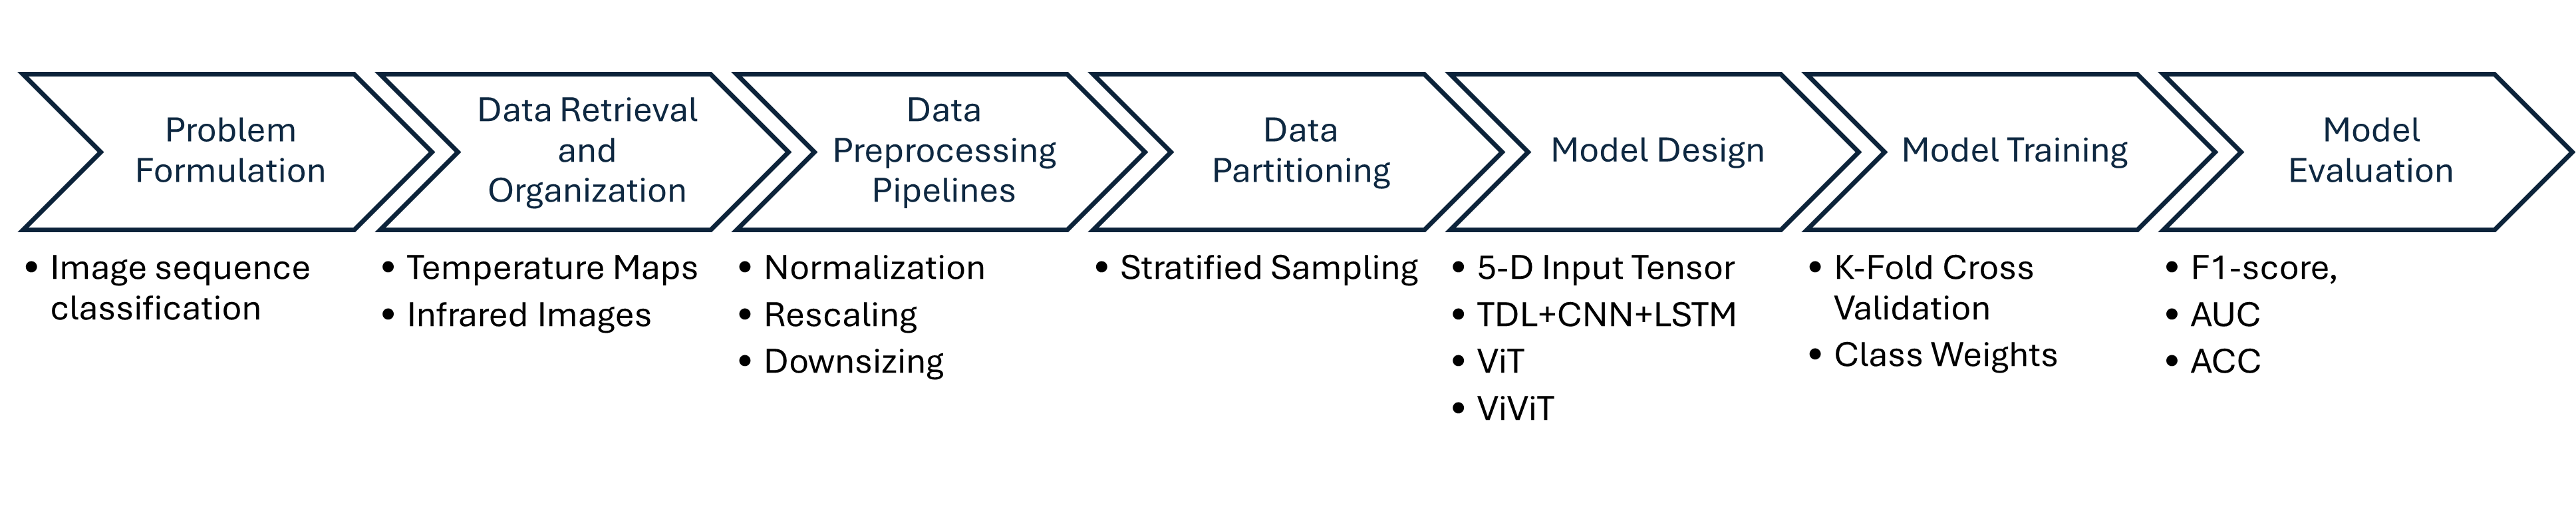
\includegraphics[width=\textwidth]{figures/methodology2.png}
  \caption{Methodology Overview \label{fig:methodoly-overview} }
\end{figure}

\subsection{Problem Formulation}
\label{sec:problem-formulation}

Our objective is to train a model to classify a sequence of \ac{TG}
data into either \textit{Benign} or \textit{Cancer}. Consequently, we
want to find a mapping function
$f_{\theta}: \mathbb{R}^{F \times C \times H \times W} \to [0,1]^B$
with parameters $\theta$, where the predicted class probabilities for
an input sequence
$\mathbf{x} \in \mathcal{X} \subset \mathbb{R}^{F \times C \times H
  \times W}$:

\begin{equation}
    \hat{y} = f_\theta(\mathbf{x}) \quad \text{(for $\mathbf{x} \in \mathcal{X}$)}
\end{equation}

Considering that a video classification aims to predict the class of a
given input sequence of frames \cite{Selva_2023}, the final prediction
$y_{pred} \in \{0,1\}^B$ is:

\begin{equation}
    y_{pred} = \mathbb{I}_{\hat{y} > 0.5}
\end{equation}
The optimization objective minimizes the binary cross-entropy loss:
\begin{equation}
    \mathcal{L}(\theta) = -\frac{1}{B}\sum_{i=1}^B \left[y_i\log(\hat{y}_i) + (1-y_i)\log(1-\hat{y}_i)\right]
\end{equation}
where $y \in \{0,1\}^B$ are the ground truth labels.

In this context, we hypothesize that  \ac{ViViTs} can outperform
3D \ac{CNNs} in \ac{BC} classification for \ac{TG}.

\subsection{Data Collection, Preprocessing and Data Augmentation}
\label{sec:dataset}

DMR-IR dataset contains \ac{TG} data of \ac{BC} patients acquired
under either the \ac{SIT} or the \ac{DIT} protocol. This data is
provided in two formats: \ac{TM} and \ac{IR}. The former comprises a
single–channel, two–dimensional matrix of floating-point temperature
values captured by the FLIR SC620 infrared camera. The latter consists
of RGB images acquired from the same camera, which offers a
measurement accuracy of \(\pm2\,^{\circ}\mathrm{C}\)
\cite{DeMatheus2023}. In both cases, the resolution is
\(640\times 480\) pixels. However, as noted in \cite{Garia2023}, the
number of subjects and images varies across studies, making direct
comparisons difficult. Table~\ref{tab:dataset_comparison} summarizes
the characteristics of \(\mathbb{D}^{\mathrm{TM}}\) and
\(\mathbb{D}^{\mathrm{IR}}\).

Even though all images in $\mathbb{D}^{\mathrm{IR}}$, are \texttt{.jpg} files,
we found that 28 cases presented images of $160 \times 120$ and 1 case of
$800 \times 600$. All of which were resized to $640 \times 480$. Also,
a total of 21 images were copies of a previous sequence. This happened
to 7 cases.


\begin{table}[h]
  \centering
  \small
\caption{DMR-IR dataset characteristics}
\label{tab:dataset_comparison}
\begin{tabular}{lcc}
% \hline
\textbf{Feature} & $\mathbb{D}^{\mathrm{TM}}$ & $\mathbb{D}^{\mathrm{IR}}$ \\
  \hline
  Type & Temperature Map & Infrared RGB Image \\
  \hline
Image size & $640 \times 480$ & $640 \times 480$ \\
Channels & 1 (Grayscale) & 3 (RGB) \\
\hline
Total patients & 55 & 149 \\
- With cancer & 36 & 87 \\
- Without cancer & 19 & 62 \\
\hline
Frames per patient & 20 & 20 \\
Total images & \numprint{1100} & \numprint{2980} \\
\hline
Training set patients & 46 & 134 \\
Test set patients & 9 & 15 \\
\hline
\end{tabular}
\end{table}

For $\mathbb{D}^{\mathrm{TM}}$, normalization was performed using the entire
patient sequence. As for the case of $\mathbb{D}^{\mathrm{IR}}$, predefined
normalization values were applied to match the requirements of the
pre-trained networks employed.  Since the \ac{DIT} protocol operates
at the patient level, the number of available samples is inherently
limited. To mitigate this constraint, data augmentation was applied
exclusively to the training fold. The augmentation strategy differs
from that of \cite{DeMatheus2023}, incorporating only the following
transformations: horizontal flip, rotation up to $15^{\circ}$, and
resize. Other augmentation techniques were excluded to preserve the
thermal properties of the data, which differ significantly from
natural images. Building upon this idea, we do not consider of use to
apply shearing transformations and introducing noise. 


% Visual Lab at the fluminense contains \ac{TG} and \ac{MG} images from voluntary
% patients. In the case of \ac{TG}, there are two protocols: dynamic and
% static. 
% \begin{lstlisting}
% wget --no-check-certificate http://visual.ic.uff.br/proeng/thiagoelias/database.rar
% \end{lstlisting}
\subsection{Model Development}
\label{sec:model-development}

Two categories of models were studied: (1) spatio-temporal
architectures, and (2) spatial-only. The former experiments with
\ac{TDL} and \ac{ViViTs}. While, the latter, applies the basic
\ac{ViT} designed to the flatten inputs (i.e.  $(B\times F, C, H)$)
without temporal modeling. Both PyTorch and Keras/Tensorflow were used
as the deep learning backends.

% Table X introduces the different models
% studied in this research with their main characteristics.

\subsubsection{Time Distributed Layer Model}
\label{sec:time-distr-layer}
Building upon the hybrid architecture proposed in \cite{Dhage2025}, we
implement a sequential model combining \ac{TDL} for spatial feature
extraction and \ac{LSTM} for temporal modeling. The network processes
input tensors
$\mathbf{x} \in \mathbb{R}^{F \times H \times W \times C}$ through
three distinct stages:

\begin{enumerate}
    \item \textbf{Spatial Feature Extraction}: Each frame undergoes:
    \begin{itemize}
        \item Resizing to $224\times224$ resolution
        \item Two convolutional blocks (32 and 16 filters, $3\times3$ kernels, ReLU)
        \item Max pooling ($2\times2$) after each convolution
        \item Batch normalization for stable training
    \end{itemize}
    
    \item \textbf{Temporal Processing}:
    \begin{itemize}
        \item Global max pooling reduces spatial dimensions to 16 features per frame
        \item LSTM layer (16 units) with $\ell_2$ regularization ($\lambda=0.01$) models temporal dynamics
    \end{itemize}
    
    \item \textbf{Classification Head}:
    \begin{itemize}
        \item Dense layer (16 units, ReLU) with $\ell_2$ regularization
        \item Dropout ($p=0.5$) for regularization
        \item Sigmoid output for binary classification
    \end{itemize}
\end{enumerate}

The \ac{TDL} wrapper enables weight sharing across all frames,
applying identical transformations to each temporal slice. Data
augmentation was carried out during training.  We employ
early stopping and model checkpointing based on validation loss,
implemented via Keras/TensorFlow. This architecture efficiently
combines:
\begin{itemize}
    \item Spatial feature learning through convolutional operations
    \item Temporal modeling via recurrent connections
    \item Regularization techniques ($\ell_2$, dropout) to prevent overfitting
\end{itemize}


This model was engineered to be small to account for the lack of
patients in the \ac{TM} dataset. It has a total of \numprint{7377}
trainable parameters. \ac{TM} were resized due to memory constrains.



\subsubsection{Basic Vision Transformer}
\label{sec:basic-visi-transf}

\ac{ViTs} are inherently spatial architectures. We designed our
\ac{ViT}-based classifier to process complete sequences of 20 thermal
frames per case, maintaining compatibility with the standard 5D input
tensor format $(B, T, C, H, W)$. We construct our model from the base
architecture proposed in \cite{dosovitskiy2020image}. The architecture
consists of:

\begin{itemize}
    \item A pretrained ViT-B/16 backbone (ImageNet1K weights) with its classification head removed
    \item Frame-wise feature extraction where:
    \begin{itemize}
        \item Input sequences are reshaped from $(B, T, C, H, W)$ to $(B \times T, C, H, W)$
        \item Each frame passes independently through the ViT encoder
        \item Features are extracted from the final layer (dimension $D=768$)
    \end{itemize}
    \item A linear classification head that:
    \begin{itemize}
        \item Projects features to logits $(B \times T, 1)$
        \item Reshapes outputs back to $(B, T, 1)$
        \item Computes temporal mean predictions $(B, 1)$
    \end{itemize}
\end{itemize}

This design enables parallel processing of all frames while preserving
sequence information through temporal averaging. The model accepts the
same 5D tensor format as traditional video architectures but leverages
ViT's superior spatial modeling capabilities for thermal image
analysis. A total of \numprint{85799425} parameters are to be
trained, when using $16 \times 16$ patches and \numprint{87456001},
when the size of the patches is increased to $32\times 32$.
\subsubsection{Video Transformer}
\label{sec:video-transformer}

Since video classification requires both spatial and temporal
processing of image sequences, we implement a TimeSformer-based
architecture \cite{Bertasius2021} for \ac{DIT}analysis. Generally,
models for video data need to address two key challenges: (1) joint
spatiotemporal feature learning, and (2) handling variable-length
sequences. However, in \ac{DIT}, this second challenge is mitigated by
the standardized protocol where each patient examination contains
exactly 20 \ac{IR} frames.

Our TimeSformerThermoClassifier consists of:

\begin{itemize}
    \item A pretrained TimeSformer-base model (finetuned on Kinetics-400) with:
    \begin{itemize}
        \item Input configuration for $T=20$ frames at $H \times W$ resolution
        \item Spatiotemporal attention across divided space-time patches
        \item Hidden dimension $D=768$ throughout all layers
    \end{itemize}
    
    \item Modified classification head:
    \begin{itemize}
        \item Original Kinetics-400 classification layer replaced
        \item Single-output linear layer for binary prediction
        \item Sigmoid activation (implicit in BCE loss)
    \end{itemize}
\end{itemize}

The forward pass processes input tensors
$\mathbf{X} \in \mathbb{R}^{B \times T \times C \times H \times W}$
through:
\begin{enumerate}
    \item Frame rearrangement (when needed) to match TimeSformer's expected $(B,C,T,H,W)$ format
    \item Spatiotemporal feature extraction via:
    \begin{itemize}
        \item Patch embedding (typically $16\times16$)
        \item Divided space-time attention layers
    \end{itemize}
    \item Global average pooling of spatiotemporal features
    \item Binary classification via the final linear layer
\end{enumerate}

This architecture leverages TimeSformer's proven effectiveness in
video understanding while adapting it specifically for thermal medical
imaging, where temporal consistency is guaranteed by the \ac{DIT}
acquisition protocol. However, the base architecture used in this
research is able to hold up to 8 frames. To account to this fact we
developed a random sampling from sequence code which allowed to
extract up to 8 frames from the 20 without altering the order of the
sequence. 




% \begin{enumerate}
% \item Review literature about \ac{CNNs} vs \ac{ViT}
% \item Check repositories about \ac{ViT}:
%   \begin{itemize}
%   \item
%     \url{https://github.com/google-research/vision\_transformer/blob/main/vit\_jax/models\_vit.py}
%   \item \url{https://github.com/Alibaba-MIIL/ImageNet21K}
%   \end{itemize}
% \end{enumerate}
\subsection{Experimental Protocol}
\label{sec:training-protocol}

Figure \ref{fig:exp-guide} presents a guide for the experiments
carried out in this research and compares the performance of the
different models on the \textit{F1-score} metric for the
\textit{K-Fold Cross Validation} strategy. Sequential models are
highlighted. 

\begin{figure}[ht]
  \centering
  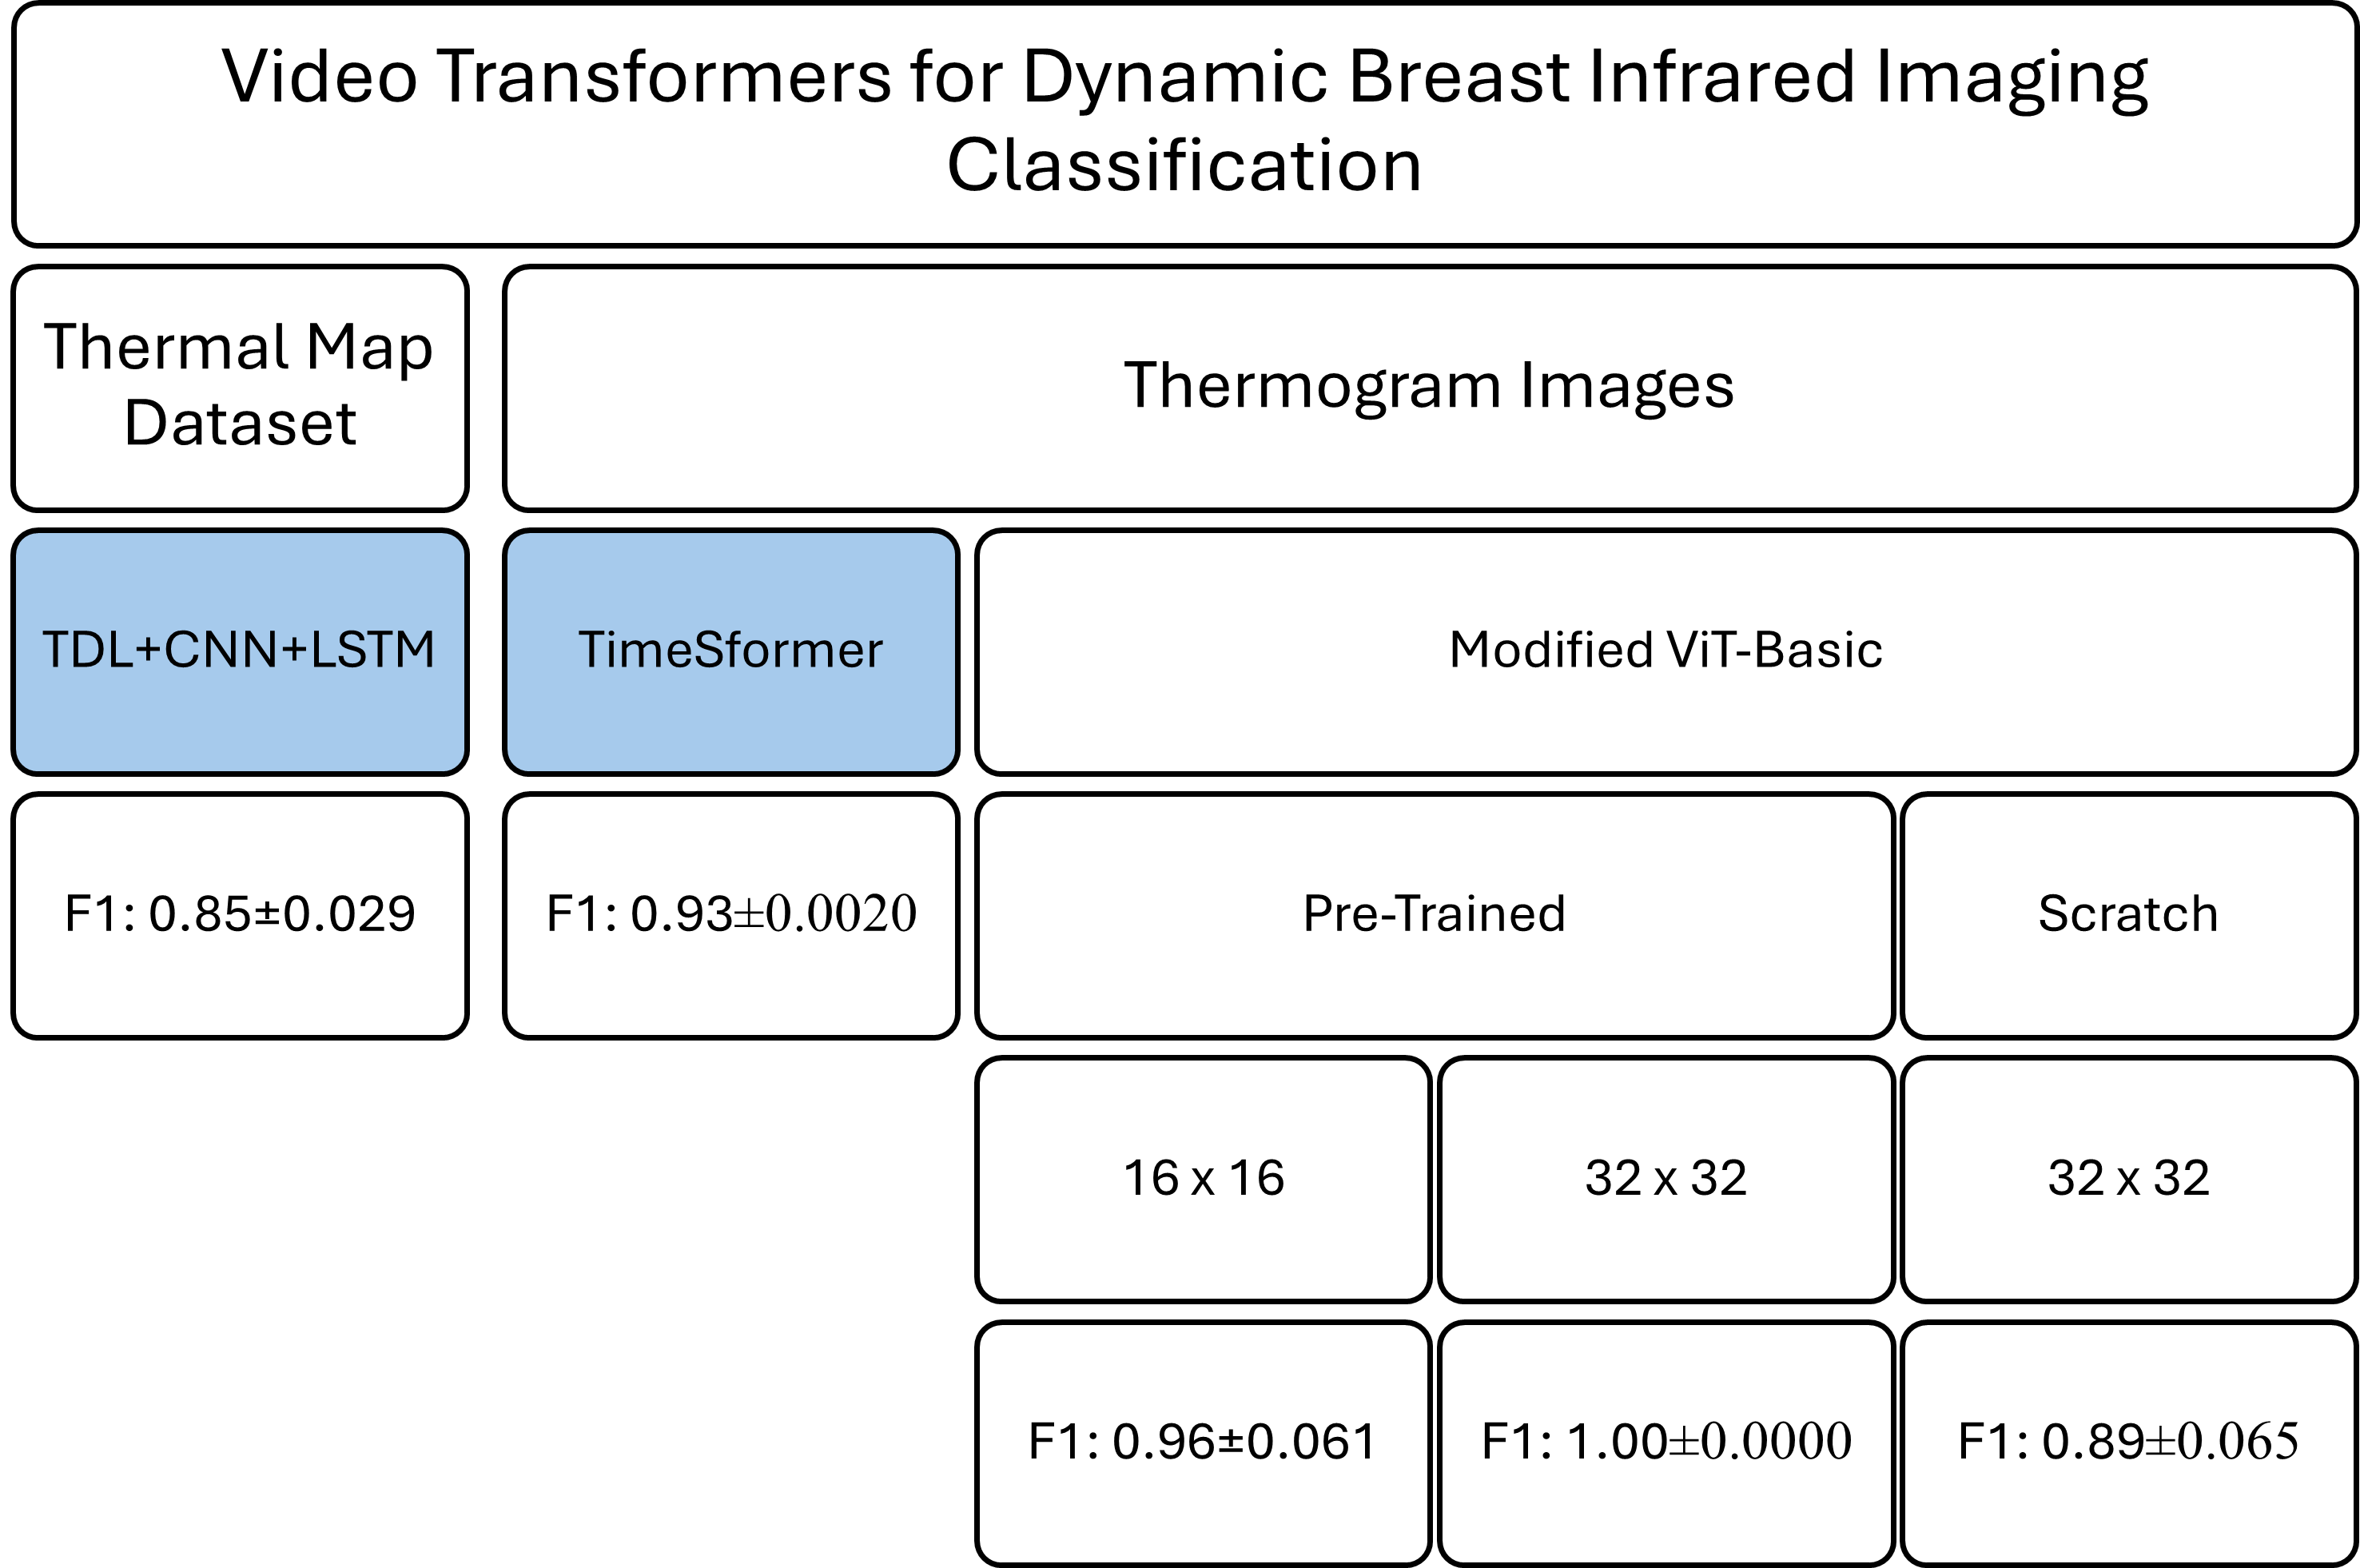
\includegraphics[scale=0.35]{figures/experimentalMethodologyGuide.png}
  \caption{F1-score performance of Models for \ac{BC} in \ac{DIT}\label{fig:exp-guide} }
\end{figure}

\begin{table}[h]
\centering
\caption{Training protocols for different modalities and architectures}
\label{tab:training_protocols}
\begin{tabular}{lllll}
\hline
\textbf{Modality} & \textbf{Model} & \textbf{Training Configuration} & \textbf{Validation} & \textbf{Epochs} \\
\hline
\ac{TM} & - & AdamW, $k=3$ CV & Loss & 50 \\
\hline
\multirow{2}{*}{\ac{IR}} & \ac{ViT} (16$\times$16) & AdamW, lr=3e-5, $k=10$ CV & F1-score & 20 \\
 & \ac{ViT} (32$\times$32) pretrained & AdamW, lr=3e-5, $k=10$ CV & F1-score & 20 \\
\hline
\ac{IR} & \ac{ViT} (32$\times$32) scratch & \begin{tabular}[c]{@{}l@{}}AdamW, lr=1e-4, wd=0.05\\ LR warmup + cosine\\ (min lr=1e-6), $k=10$ CV\end{tabular} & Loss & 50 \\
\hline
\ac{IR} & \ac{ViViT} & AdamW, lr=3e-5, $k=10$ CV & F1-score & 20 \\
\hline
\end{tabular}
\end{table}

Our experimental protocol varied across modalities and
architectures. For \ac{TM} data, we employed 3-fold cross-validation
trained for 50 epochs using AdamW optimizer while monitoring
validation loss. For \ac{IR} data with pretrained \ac{ViT} models
(both 16$\times$16 and 32$\times$32 patch sizes), we used 10-fold
cross-validation for 20 epochs with a learning rate of 3e-5,
optimizing for validation F1-score. However, when training the
32$\times$32 patch \ac{ViT} from scratch, we extended training to 50
epochs with higher initial learning rate (1e-4), weight decay (0.05),
and implemented learning rate warmup with cosine annealing (minimum
lr=1e-6), while monitoring validation loss. The \ac{ViViT} model
followed similar configuration to pretrained \ac{ViT}s (20 epochs,
lr=3e-5) with F1-score monitoring.

% \begin{enumerate}
% \item Replicate results provided in \cite{Garia2023} to assess that
%   training from scratch a \ac{ViT} achieves the reported performance in
%   static \ac{TG} images.
% \item Fine Tune a model using the same dataset
% \item Extend model for dynamic dataset
% \end{enumerate}

\subsection{Evaluation Metrics}
\label{sec:evaluation-metrics}

In this research we used the following evaluation metrics to study the
performance of the models in both datasets:

\begin{itemize}
    \item \textbf{Accuracy}: Measures overall prediction correctness:
    \[
    \text{Accuracy} = \frac{TP + TN}{TP + TN + FP + FN}
    \]
    where $TP$, $TN$, $FP$, and $FN$ denote true positives, true negatives, false positives, and false negatives respectively.

    \item \textbf{F1-score}: Harmonic mean of precision and recall:
    \[
    \text{F1} = 2 \times \frac{\text{Precision} \times \text{Recall}}{\text{Precision} + \text{Recall}}
    \]
    Balances false positives and false negatives, ideal for imbalanced datasets.

    \item \textbf{AUC-ROC}: Area Under the Receiver Operating Characteristic curve:
    \[
    \text{AUC} = \int_0^1 TPR(FPR) \, dFPR
    \]
    Measures model's ability to distinguish classes across all thresholds (1 = perfect, 0.5 = random).
\end{itemize}

\section{Results}
\label{sec:results}
% **Results:** Present quantitative performance (tables and figures),
% comparative analysis, and discussion.
In this section, we discuss the quantitative performance of the
different models and experiments.

\begin{table}[h]
\centering
\caption{Performance comparison of different models on \ac{DIT} data}
\label{tab:results}
\begin{tabular}{lllll}
\hline
\textbf{Modality} & \textbf{Model} & \textbf{Metric} & \textbf{Cross-Val (Mean $\pm$ Std)} & \textbf{Test Set} \\
\hline
\multirow{2}{*}{\ac{TM}} & \multirow{2}{*}{TDL+CNN+LSTM} & F1-score & $0.8585 \pm 0.0296$ ($k=3$) & - \\
 & & AUC & - & - \\
\hline
\multirow{12}{*}{\ac{IR}} & \multirow{3}{*}{ViT (16$\times$16)} & F1-score & $0.9644 \pm 0.0458$ & - \\
 & & Accuracy & $0.9538 \pm 0.0615$ & 0.87 \\
 & & AUC & - & - \\
\cline{2-5}
 & \multirow{3}{*}{ViT (32$\times$32)} & F1-score & $1.0000 \pm 0.0000$ & 0.9412 \\
 & & Accuracy & $1.0000 \pm 0.0000$ & 0.9333 \\
 & & AUC & $1.0000 \pm 0.0000$ & 0.9444 \\
\cline{2-5}
 & \multirow{3}{*}{ViT (32$\times$32)*} & F1-score & $0.9101 \pm 0.0665$ & 0.8889 \\
 & & Accuracy & $0.8939 \pm 0.0652$ & 0.8667 \\
 & & AUC & $0.8866 \pm 0.0595$ & 0.8611 \\
\cline{2-5}
 & \multirow{3}{*}{ViViT} & F1-score & $0.9339 \pm 0.0020$ & 0.9412 \\
 & & Accuracy & $0.9231 \pm 0.0000$ & 0.9333 \\
 & & AUC & $0.9350 \pm 0.0094$ & 0.9444 \\
\cline{2-5}
 & \multirow{1}{*}{3D-CNN} & AUC & $0.9351 \pm 0.0403$ & - \\
\hline
\end{tabular}
\end{table}

\begin{itemize}
    \item[*] Model trained from scratch
    \item All cross-validation results use $k=10$ unless noted
    \item Test set evaluations use 15 patients for \ac{IR} models
    \item Standard deviation for De Matheus et al. corrected to 0.0403 (4.03\% as decimal)
\end{itemize}

*Trained from scratch. All cross-validation results use $k=10$ unless
noted. Test set evaluations use 15 patients for \ac{IR} models.
\section{Conclusions}
\label{sec:conclusions}

The presented work presents, to the best of our knowledge, the first
application of a \ac{ViViT} to the \ac{DIT} protocol. We have been
able to outperform the results in \cite{DeMatheus2023} in a test set
of 15 patients and to obtain similar results to them in $K=10$ cross
validation. Also, the experiments confirm the statement in
\cite{Garia2023} about a better performance when using \ac{ViTs} with
$32 \times 32$ patches. However, it must be noticed that
\cite{Garia2023} work in \ac{SIT} protocol, while we focus on
\ac{DIT}. Different to their result, training from scratch performed
lower. Consequently, we infer that \ac{ViViTs} can be applied with a
good performance in \ac{BC} classification with \ac{TG} images.Our
experiments also suggest that future works should emphasize on what
type of thermal data was used in the experiments since results using
\ac{TM} are different from those when using \ac{IR} images.
% **Conclusions:** Summarize findings, state contributions, and
% mention limitations.
% \section{Future Works}
% \label{sec:future-works}
% **Future Works:** Suggest improvements, possible applications, and
% further research directions.



% \section{First Section}
% \subsection{A Subsection Sample}
% Please note that the first paragraph of a section or subsection is
% not indented. The first paragraph that follows a table, figure,
% equation etc. does not need an indent, either.

% Subsequent paragraphs, however, are indented.

% \subsubsection{Sample Heading (Third Level)} Only two levels of
% headings should be numbered. Lower level headings remain unnumbered;
% they are formatted as run-in headings.

% \paragraph{Sample Heading (Fourth Level)}
% The contribution should contain no more than four levels of
% headings. Table~\ref{tab1} gives a summary of all heading levels.

% % ==================== tables example ====================
% \begin{table}
% \caption{Table captions should be placed above the
% tables.}\label{tab1}
% \begin{tabular}{|l|l|l|}
% \hline
% Heading level &  Example & Font size and style\\
% \hline
% Title (centered) &  {\Large\bfseries Lecture Notes} & 14 point, bold\\
% 1st-level heading &  {\large\bfseries 1 Introduction} & 12 point, bold\\
% 2nd-level heading & {\bfseries 2.1 Printing Area} & 10 point, bold\\
% 3rd-level heading & {\bfseries Run-in Heading in Bold.} Text follows & 10 point, bold\\
% 4th-level heading & {\itshape Lowest Level Heading.} Text follows & 10 point, italic\\
% \hline
% \end{tabular}
% \end{table}

% % ==================== tables example ====================
% % ==================== equations example ====================
% \noindent Displayed equations are centered and set on a separate
% line.
% \begin{equation}
% x + y = z
% \end{equation}
% Please try to avoid rasterized images for line-art diagrams and
% schemas. Whenever possible, use vector graphics instead (see
% Fig.~\ref{fig1}).
% % ==================== equations example ====================
% % ==================== figures example ====================
% \begin{figure}
% \includegraphics[width=\textwidth]{fig1.eps}
% \caption{A figure caption is always placed below the illustration.
% Please note that short captions are centered, while long ones are
% justified by the macro package automatically.} \label{fig1}
% \end{figure}
% % ==================== theorems ====================
% \begin{theorem}
% This is a sample theorem. The run-in heading is set in bold, while
% the following text appears in italics. Definitions, lemmas,
% propositions, and corollaries are styled the same way.
% \end{theorem}
% %
% % the environments 'definition', 'lemma', 'proposition', 'corollary',
% % 'remark', and 'example' are defined in the LLNCS documentclass as well.
% %
% \begin{proof}
% Proofs, examples, and remarks have the initial word in italics,
% while the following text appears in normal font.
% \end{proof}
% % ==================== theorems ====================
% % ==================== citations ====================
% For citations of references, we prefer the use of square brackets
% and consecutive numbers. Citations using labels or the author/year
% convention are also acceptable. The following bibliography provides
% a sample reference list with entries for journal
% articles~\cite{ref_article1}, an LNCS chapter~\cite{ref_lncs1}, a
% book~\cite{ref_book1}, proceedings without editors~\cite{ref_proc1},
% and a homepage~\cite{ref_url1}. Multiple citations are grouped
% \cite{ref_article1,ref_lncs1,ref_book1},
% \cite{ref_article1,ref_book1,ref_proc1,ref_url1}.
% % ==================== citations ====================
% % ==================== credits ====================
\begin{credits}
\subsubsection{\ackname} A bold run-in heading in small font size at the end of the paper is
used for general acknowledgments, for example: This study was funded
by X (grant number Y).

\subsubsection{\discintname}
It is now necessary to declare any competing interests or to specifically
state that the authors have no competing interests. Please place the
statement with a bold run-in heading in small font size beneath the
(optional) acknowledgments\footnote{If EquinOCS, our proceedings submission
system, is used, then the disclaimer can be provided directly in the system.},
for example: The authors have no competing interests to declare that are
relevant to the content of this article. Or: Author A has received research
grants from Company W. Author B has received a speaker honorarium from
Company X and owns stock in Company Y. Author C is a member of committee Z.
\end{credits}
% ==================== credits ====================
% 
% ---- Bibliography ----
%
% BibTeX users should specify bibliography style 'splncs04'.
% References will then be sorted and formatted in the correct style.
%
\bibliographystyle{splncs04}
\bibliography{bibliography}
%
% \begin{thebibliography}{8}
% \bibitem{ref_article1}
% Author, F.: Article title. Journal \textbf{2}(5), 99--110 (2016)

% \bibitem{ref_lncs1}
% Author, F., Author, S.: Title of a proceedings paper. In: Editor,
% F., Editor, S. (eds.) CONFERENCE 2016, LNCS, vol. 9999, pp. 1--13.
% Springer, Heidelberg (2016). \doi{10.10007/1234567890}

% \bibitem{ref_book1}
% Author, F., Author, S., Author, T.: Book title. 2nd edn. Publisher,
% Location (1999)

% \bibitem{ref_proc1}
% Author, A.-B.: Contribution title. In: 9th International Proceedings
% on Proceedings, pp. 1--2. Publisher, Location (2010)

% \bibitem{ref_url1}
% LNCS Homepage, \url{http://www.springer.com/lncs}, last accessed 2023/10/25
% \end{thebibliography}

\end{document}

%%% Local Variables:
%%% mode: LaTeX
%%% TeX-master: t
%%% End:
